\section{The lattice and one chain through it}
\label{sec:lattice}

A consistency model is a predicate over histories, characterized by the set of
anomalies it excludes~\cite{Adya1999}. With
$\mathcal{A}=\{A_1,A_2,A_3,A_6\}$ the design space is the Boolean lattice
$\langle 2^{\mathcal{A}},\subseteq\rangle$: sixteen points, bottom
$\emptyset$ admitting everything, top $\mathcal{A}$ admitting nothing
(\cref{fig:lattice}). We name five points on one maximal chain,
\[
  L_0\equiv\emptyset,\;
  L_1\equiv\{A_1\},\;
  L_2\equiv\{A_1,A_3\},\;
  L_3\equiv\{A_1,A_3,A_6\},\;
  L_4\equiv\mathcal{A},
\]
chosen on operational grounds (\A1 first because it is the basic
read--generate--commit failure; \A2 last because registry stability across
the operation lifetime is the costliest single requirement); the other
twenty-three linearizations are equally valid and the lattice, not the chain,
is primary. The residue predicate \Rp{} is not a generator: it is not an
anomaly, and its answer, the basis ledger $\ell$ of \cref{sec:ledger},
composes with any point.

\begin{figure}[t]
\centering
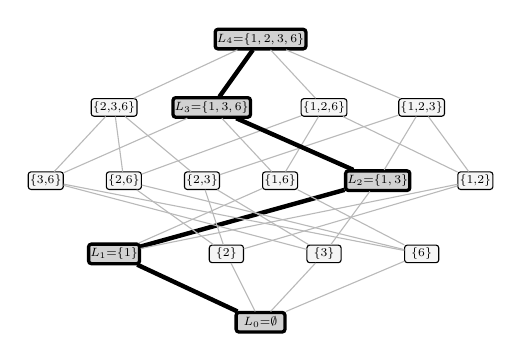
\begin{tikzpicture}[
    every node/.style={font=\scriptsize},
    pt/.style={draw, rounded corners=1pt, fill=gray!8, minimum width=7mm, minimum height=3.6mm, inner sep=1pt},
    chosen/.style={draw=black, very thick, fill=gray!35, rounded corners=1pt, minimum width=10mm, minimum height=4mm, inner sep=1pt},
    edge/.style={-, thin, gray!55},
    chosenedge/.style={-, ultra thick, black},
    scale=0.62, transform shape]
\node[chosen] (L4) at (4.0, 5.4) {$L_4{=}\{1,2,3,6\}$};
\node[pt]     (n3a) at (1.0, 4.0) {\{2,3,6\}};
\node[chosen] (L3)  at (3.0, 4.0) {$L_3{=}\{1,3,6\}$};
\node[pt]     (n3c) at (5.3, 4.0) {\{1,2,6\}};
\node[pt]     (n3d) at (7.3, 4.0) {\{1,2,3\}};
\node[pt]     (n2a) at (-0.4, 2.5) {\{3,6\}};
\node[pt]     (n2b) at (1.2, 2.5) {\{2,6\}};
\node[pt]     (n2c) at (2.8, 2.5) {\{2,3\}};
\node[pt]     (n2d) at (4.4, 2.5) {\{1,6\}};
\node[chosen] (L2)  at (6.4, 2.5) {$L_2{=}\{1,3\}$};
\node[pt]     (n2f) at (8.4, 2.5) {\{1,2\}};
\node[chosen] (L1)  at (1.0, 1.0) {$L_1{=}\{1\}$};
\node[pt]     (n1b) at (3.3, 1.0) {\{2\}};
\node[pt]     (n1c) at (5.3, 1.0) {\{3\}};
\node[pt]     (n1d) at (7.3, 1.0) {\{6\}};
\node[chosen] (L0) at (4.0, -0.4) {$L_0{=}\emptyset$};
\draw[chosenedge] (L0) -- (L1); \draw[edge] (L0) -- (n1b); \draw[edge] (L0) -- (n1c); \draw[edge] (L0) -- (n1d);
\draw[edge] (L1) -- (n2d); \draw[chosenedge] (L1) -- (L2); \draw[edge] (L1) -- (n2f);
\draw[edge] (n1b) -- (n2b); \draw[edge] (n1b) -- (n2c); \draw[edge] (n1b) -- (n2f);
\draw[edge] (n1c) -- (n2a); \draw[edge] (n1c) -- (n2c); \draw[edge] (n1c) -- (L2);
\draw[edge] (n1d) -- (n2a); \draw[edge] (n1d) -- (n2b); \draw[edge] (n1d) -- (n2d);
\draw[edge] (n2a) -- (n3a); \draw[edge] (n2a) -- (L3); \draw[edge] (n2b) -- (n3a); \draw[edge] (n2b) -- (n3c);
\draw[edge] (n2c) -- (n3a); \draw[edge] (n2c) -- (n3d); \draw[edge] (n2d) -- (L3); \draw[edge] (n2d) -- (n3c);
\draw[chosenedge] (L2) -- (L3); \draw[edge] (L2) -- (n3d); \draw[edge] (n2f) -- (n3c); \draw[edge] (n2f) -- (n3d);
\draw[edge] (n3a) -- (L4); \draw[chosenedge] (L3) -- (L4); \draw[edge] (n3c) -- (L4); \draw[edge] (n3d) -- (L4);
\end{tikzpicture}
\caption{The lattice $\langle 2^{\{A_1,A_2,A_3,A_6\}},\subseteq\rangle$
(sets abbreviated by index) and the chain realized by verified runtimes
(bold). Every point is realized by the parameterized runtime of
\cref{sec:lattice16}, with or without the basis ledger.}
\label{fig:lattice}
\end{figure}

\subsection{What is and is not a result}
The chain's inclusions are definitional and its strictness needs one witness
per step; neither is a result. What requires work is \emph{realizability}: a
runtime configuration that excludes exactly each point's anomalies, and for
the five named points a verified realizing runtime---established here by
bounded model checking, and claimed at the bounds stated.

\subsection{All sixteen points, mechanically; the ledger composes}
\label{sec:lattice16}
\texttt{Guarded.tla} extends the runtime with four commit-time disciplines,
each enabled by a Boolean constant and each acting on its own carrier: $G_1$,
read-set validation (an operation whose read set was overwritten after its
read may not commit); $G_2$, registry validation (a planned tool no longer in
the registry may not be dispatched); $G_3$, causal tracking with output commit
(an operation records the closure of committed writers whose values it read,
may not commit while any is aborted, externalizes only once its closure has
externalized, and once externalized is irrevocable; a retraction cascades to
every unexternalized dependent); $G_6$, commit-order sequencing (effects
externalize in issuance order). The carriers are disjoint---read set and write
times; registry and planned tool; closure and abort flags; issuance and commit
orders---so enabling one guard neither creates nor removes another anomaly,
and the matrix confirms it on every combination.

For each of the sixteen guard sets $S$ and each anomaly $a$, TLC checks
$R(S)\models\neg a$: for $a\in S$ the invariant must hold exhaustively, for
$a\notin S$ it must be violated. All \LatticeRuns{} runs match
(\texttt{lattice16.sh}; $|A|{=}2$, $|\fld{Cells}|{=}2$, $|\fld{Values}|{=}1$,
$\fld{MaxOps}{=}2$, symmetry on agents and cells; the $32$ safety runs are
exhaustive over \LatticeSafeStatesMin{}--\LatticeSafeStatesMax{} distinct
states). Because \textsc{CausalCascade} ranges over flags and predecessor
sets and never over cells, the sixteen \textsc{NoA3} points are rechecked at
$\fld{MaxOps}{=}3$ with one cell, where a transitive cascade first becomes
reachable: \LatticeMaxOpsThreeRuns{}/\LatticeMaxOpsThreeRuns{} match. A
single-value domain makes \cref{def:a1}'s value conjunct vacuous on non-null
reads; the safety half re-run at $|\fld{Values}|{=}2$ stays safe in all
$32$ cells, and a targeted check shows the non-null-read witness class needs
both a second value \emph{and} a third operation (supplement \S\,L); the
two-value safety half is re-run on the current model (\LatticeVtwoOutcome).
Every point is thus inhabited by a runtime that prevents exactly its
avoidance set, at these bounds; the Verus product of the $L_2$, $L_3$ and
$L_4$ models (\cref{sec:composition}) mechanizes the top point without a
bound.

\smallskip\noindent\emph{The ledger composes.} \texttt{Guarded5.tla} adds a
fifth constant $G_7$, the basis ledger of \cref{sec:ledger}, which refuses
nothing and writes only the basis and obligation fields.
\texttt{lattice32.sh} runs all \LatticeThirtyTwoRuns{} combinations of the
five constants against the four anomalies and \Rp{} at the same bounds. The
$64$ anomaly cells with $G_7$ on return the verdicts of \texttt{lattice16.sh}
one for one, so the ledger disturbs no point of the lattice; \Rp{} is
reached without $G_7$ in a five-state trace at every point and excluded
with $G_7$ at every point (exhaustive; \NoAsevenStates{} distinct states at
the bottom point, \NoAsevenStatesGthree{} with output commit, where a held
effect can be superseded before its release). \LatticeThirtyTwoOutcome{}
